\documentclass[a4paper]{article}

\usepackage{../header}
\setlength{\parskip}{1em}
\setlength\parindent{2em}

\newcommand{\spec}{\operatorname{spec}}
\newcommand{\tr}{\operatorname{tr}}
\newcommand{\rk}{\operatorname{rk}}

\title{\HugeЛАИГ. Летний экзамен}
\author{
    \href{https://teleg.run/lodthe}{Балюк Игорь}, 193 группа
}

\begin{document}
    \maketitle
    \tableofcontents
    
    \newpage
    \section{Изменение матрицы линейного оператора при переходе к другому базису: П1452--1454; К 39.19--39.21.}

        Тут главное знать, что если у нас был переход от базиса $e$ к базису $f$:
        \begin{equation*}
            f = e \cdot C,
        \end{equation*}
        то матрицу линейного оператора можно найти по следующей формуле:
        \begin{equation*}
            A(\phi, f, f) = C^{-1} \cdot A(\phi, e, e) \cdot C.
        \end{equation*}

    \begin{enumerate}
    \item[\textbf{П1452}]
        Линейное преобразование $\phi$ в базисе $e_1, e_2, e_3, e_4$ имеет матрицу
        \begin{equation*}
            A = \begin{pmatrix}
                1 & 2 & 0 & 1 \\
                3 & 0 & -1 & 2 \\
                2 & 5 & 3 & 1 \\
                1 & 2 & 1 & 3 \\
            \end{pmatrix}.
        \end{equation*}

        Найти матрицу этого же преобразования в базисе
        \begin{options}
        \item $e_1, e_3, e_2, e_4$;
            \begin{solution}
                Пристальным взглядом понимаем, что здесь меняются вторая и третья строка и второй и третий столбец. Новая матрица имеет следующий вид:
                \begin{equation*}
                    \begin{pmatrix}
                        1 & 0 & 2 & 1 \\
                        2 & 3 & 5 & 1 \\
                        3 & -1 & 0 & 2 \\
                        1 & 1 & 2 & 3 \\
                    \end{pmatrix}.
                \end{equation*}
            \end{solution}

        \item $e_1, e_1 + e_2, e_1 + e_2 + e_3, e_1 + e_2 + e_3 + e_4$.
            \begin{solution}
                Матрица перехода от старого базиса к новому:
                \begin{equation*}
                    C = \begin{pmatrix}
                        1 & 1 & 1 & 1 \\
                        0 & 1 & 1 & 1 \\
                        0 & 0 & 1 & 1 \\
                        0 & 0 & 0 & 1 \\
                    \end{pmatrix}.
                \end{equation*}

                Тогда в новом базисе матрица имеет следующий вид:
                \begin{equation*}
                    C^{-1} \cdot A \cdot C = 
                    \begin{pmatrix}
                        1 & -1 & 0 & 0 \\
                        0 & 1 & -1 & 0 \\
                        0 & 0 & 1 & -1 \\
                        0 & 0 & 0 & 1 \\
                    \end{pmatrix}
                    \cdot
                    \begin{pmatrix}
                        1 & 2 & 0 & 1 \\
                        3 & 0 & -1 & 2 \\
                        2 & 5 & 3 & 1 \\
                        1 & 2 & 1 & 3 \\
                    \end{pmatrix}
                    \cdot
                    \begin{pmatrix}
                        1 & 1 & 1 & 1 \\
                        0 & 1 & 1 & 1 \\
                        0 & 0 & 1 & 1 \\
                        0 & 0 & 0 & 1 \\
                    \end{pmatrix}
                    =
                    \begin{pmatrix}
                        -2 & 0 & 1 & 0 \\
                        1 & -4 & -8 & -7 \\
                        1 & 4 & 6 & 4 \\
                        1 & 3 & 4 & 7 \\
                    \end{pmatrix}.
                \end{equation*}
            \end{solution}
        \end{options}

    \item[\textbf{П1454}]
        Линейное преобразование $\phi$ в базисе $a_1 = (8, -6, 7), a_2 = (-16, 7, -13), a_3 = (9, -3, 7)$ имеет матрицу
        \begin{equation*}
            \begin{pmatrix}
                1 & -18 & 15 \\
                -1 & -22 & 20 \\
                1 & -25 & 22 \\
            \end{pmatrix}.
        \end{equation*}

        Найдите его матрицу в базисе
        \begin{equation*}
            b_1 = (1, -2, 1); \quad
            b_2 = (3, -1, 2); \quad
            b_3 = (2, 1, 2).
        \end{equation*}

        \begin{solution}
            Здесь у нас заранее неясна матрица перехода. Она находится решением уравнения $(a_1 | a_2 | a_3 |) \cdot X = (b_1 | b_2 | b_3)$. Дальше находим матрицу линейного оператора в новом базисе по формуле выше.
        \end{solution}

    \item[\textbf{К39.20}]
        Пусть линейный оператор в пространстве $\RR[x]_2$ имеет в базисе $(1, x, x^2)$ матрицу
        \begin{equation*}
            \begin{pmatrix}
                0 & 0 & 1 \\
                0 & 1 & 0 \\
                1 & 0 & 0 \\
            \end{pmatrix}.
        \end{equation*}

        Найдите его матрицу в базисе
        \begin{equation*}
            (3x^2 + 2x + 1, x^2 + 3x + 2, 2x^2 + x + 3).
        \end{equation*}

        \begin{solution}
            Здесь надо сказать, что каждому многочлену однозначно сопоставляется вектор с его коэффициентами:
            \begin{equation*}
                a + bx + cx^2 \mapsto (a, b, c).
            \end{equation*}
            
            Переходим к привычным нам векторам, считаем ответ.
        \end{solution}
    \end{enumerate}
    
    \newpage
    \section{Собственные векторы и собственные значения линейных операторов: П 1465--1474; К 40.15.}

    Алгоритм решения такой задачи Дима уже описал \href{https://docviewer.yandex.ru/view/286099993/?*=1y%2B9IzuiXNOrJ6ZQ01NuoVUurxt7InVybCI6InlhLWRpc2stcHVibGljOi8vNVhNeGdORnVtNjBWcGRJV04vVzdCbTYzMU9POUZCYUswWktLSWxGVk85aG96dCt3Zlg4Q2pOcCs0NWpHMnh4Q3EvSjZicG1SeU9Kb25UM1ZvWG5EYWc9PTovU2VtaW5hcjI5X2FsZ29yaXRobXMucGRmIiwidGl0bGUiOiJTZW1pbmFyMjlfYWxnb3JpdGhtcy5wZGYiLCJub2lmcmFtZSI6ZmFsc2UsInVpZCI6IjI4NjA5OTk5MyIsInRzIjoxNTkxNzQwMTg3OTA0LCJ5dSI6IjU0Mjk1MDEzNDE1NjU1MjYzNjIifQ%3D%3D}{здесь}.

    \begin{enumerate}
    \item[\textbf{К40.15в}]
        Найти собственные значения и собственные векторы линейных операторов, заданных в некотором базисе матрицей
        \begin{equation*}
            \begin{pmatrix}
                4 & -5 & 2 \\
                5 & -7 & 3 \\
                6 & -9 & 4 \\
            \end{pmatrix}.
        \end{equation*}

        \begin{solution}
            Найдем собственные значения. Они являются корнями многочлена $(-1)^n \chi_A(\lambda) = \det(A~-~\lambda E)$:
            \begin{equation*}
                \det(A - \lambda E) = \begin{vmatrix}
                    4 - \lambda & -5 & 2 \\
                    5 & -7 - \lambda & 3 \\
                    6 & -9 & 4 - \lambda \\
                \end{vmatrix}
                = x^2 - x^3 = x^2(1 - x) \implies \spec{A} = \{0, 1\}.
            \end{equation*}

            Зная собственные значения, можно найти ФСР, которые будут задавать собственное подпространство:
            \begin{itemize}
            \item[\pmb{$\lambda_1 = 0$}]
                \[\begin{gathered}
                    \begin{amatrix}{3}{1}
                        4 & -5 & 2 & 0 \\
                        5 & -7 & 3 & 0 \\
                        6 & -9 & 4 & 0 \\
                    \end{amatrix}
                    \to
                    \begin{amatrix}{3}{1}
                        1 & -2 & 1 & 0 \\
                        0 & 3 & -2 & 0 \\
                        0 & 3 & -2 & 0 \\
                    \end{amatrix}
                    \to
                    \begin{amatrix}{3}{1}
                        3 & 0 & -1 & 0 \\
                        0 & 3 & -2 & 0 \\
                        0 & 0 & 0 & 0 \\
                    \end{amatrix}
                    \implies V_{0}(A) = \langle (1/3, 2/3, 1) \rangle.
                \end{gathered}\]

            \item[\pmb{$\lambda_2 = 0$}]
                Случай, аналогичный предыдущему пункту.

            \item[\pmb{$\lambda_3 = 1$}]
                \[\begin{gathered}
                    \begin{amatrix}{3}{1}
                        3 & -5 & 2 & 0 \\
                        5 & -8 & 3 & 0 \\
                        6 & -9 & 3 & 0 \\
                    \end{amatrix}
                    \to
                    \begin{amatrix}{3}{1}
                        1 & -1 & 0 & 0 \\
                        0 & -2 & 2 & 0 \\
                        0 & -3 & 3 & 0 \\
                    \end{amatrix}
                    \to
                    \begin{amatrix}{3}{1}
                        1 & 0 & -1 & 0 \\
                        0 & 1 & -1 & 0 \\
                        0 & 0 & 0 & 0 \\
                    \end{amatrix}
                    \implies V_{1}(A) = \langle (1, 1, 1) \rangle.
                \end{gathered}\]
            \end{itemize}

            Собственными значениями являются $0$, $0$ и $1$. Им соответствуют собственные векторы вида $k \cdot (1, 2, 3)$, $k \cdot (1, 2, 3)$ и $k \cdot (1, 1, 1)$ соответственно (где $k \neq 0$).
        \end{solution}
    \end{enumerate}
    
    \newpage
    \section{Диагонализуемость линейных операторов: П 1479--1483; К 40.16.}
    Алгоритм решения такой задачи Дима уже описал \href{https://docviewer.yandex.ru/view/286099993/?*=1y%2B9IzuiXNOrJ6ZQ01NuoVUurxt7InVybCI6InlhLWRpc2stcHVibGljOi8vNVhNeGdORnVtNjBWcGRJV04vVzdCbTYzMU9POUZCYUswWktLSWxGVk85aG96dCt3Zlg4Q2pOcCs0NWpHMnh4Q3EvSjZicG1SeU9Kb25UM1ZvWG5EYWc9PTovU2VtaW5hcjI5X2FsZ29yaXRobXMucGRmIiwidGl0bGUiOiJTZW1pbmFyMjlfYWxnb3JpdGhtcy5wZGYiLCJub2lmcmFtZSI6ZmFsc2UsInVpZCI6IjI4NjA5OTk5MyIsInRzIjoxNTkxNzQwMTg3OTA0LCJ5dSI6IjU0Mjk1MDEzNDE1NjU1MjYzNjIifQ%3D%3D}{здесь}.

    Вспоминаем критерий диагонализуемости оператора. Оператор диагонализуем, если его характеристический многочлен разлагается на произведение линейных множителей и алгебраическая кратность равна геометрической кратности для всех собственных значений.

    То есть если мы не можем представить характеристический многочлен в виде произведения линейных множителей, можно сразу сказать,что оператор не диагонализуем. Иначе придется находить собственные векторы. Если геометрическая кратность (размерность собственного подпространства) будет равна алгебраической кратности (степень, с которой линейных множитель входит в разложение) для каждого собственного значения, то оператор будет диагонализуем, а в диагональном виде матрицы на диагонали будут записаны собственные значения.

    Выяснить, какие из следующих матриц линейных преобразований можно привести к диагональному виду путем перехода к новому базису. Найти этот базис и соответствующую ему матрицу:
    \begin{options}
    \item[\textbf{П1479}]
        \begin{equation*}
            A = \begin{pmatrix}
                -1 & 3 & -1 \\
                -3 & 5 & -1 \\
                -3 & 3 & 1 \\
            \end{pmatrix}.
        \end{equation*}

        \begin{solution}
            Найдем характеристический многочлен
            \begin{equation*}
                \chi_{\phi} = (-1)^{3} \cdot \det{A - tE} = 
                (-1)^3 \cdot
                \begin{vmatrix}
                    -1 - t & 3 & -1 \\
                    -3 & 5 - t & -1 \\
                    -3 & 3 & 1 - t \\
                \end{vmatrix}
                = t^3 - 5t^2 + 8t - 4
                = (t - 2)^2 \cdot (t - 1).
            \end{equation*}

            Найдем собственные векторы для найденных собственных значений.
            \begin{itemize}
            \item[\pmb{$t_1 = 1$}]
                Найдем ФСР у $(A - 1 \cdot E) \cdot x = 0$. Это система из одного вектора: $((1, 1, 1))$. Любопытный читатель может сделать это руками.

            \item[\pmb{$t_2 = t_3 = 2$}]
                Найдем ФСР у $(A - 2 \cdot E) \cdot x = 0$. Это система $((1, 1, 0), (-1/3, 0, 1))$.
            \end{itemize}

            Так как $a_1 = 1 = g_1$ и $a_2 = 2 = g_2$ и мы нашли разложение характеристического многочлена на линейные множители, оператор диагонализуем. Его матрица принимает диагональный вид
            \begin{equation*}
                \begin{pmatrix}
                    1 & 0 & 0 \\
                    0 & 2 & 0 \\
                    0 & 0 & 2 \\
                \end{pmatrix}
            \end{equation*}
            в следующем базисе:
            \begin{equation*}
                (1, 1, 1), (1, 1, 0), (-1/3, 0, 1).
            \end{equation*}
        \end{solution}

    \item[\textbf{П1480}]
        \begin{equation*}
            \begin{pmatrix}
                6 & -5 & -3 \\
                3 & -2 & -2 \\
                2 & -2 & 0 \\
            \end{pmatrix}.
        \end{equation*}

        \begin{solution}
            Найдем характеристический многочлен
            \begin{equation*}
                \chi_{\phi} = (-1)^{3} \cdot \det{A - tE} = 
                (-1)^3 \cdot
                \begin{vmatrix}
                    6 - t & -5 & -3 \\
                    3 & -2 - t & -2 \\
                    2 & -2 & -t \\
                \end{vmatrix}
                = t^3 - 4t^2 + 5t - 2
                = (t - 2) \cdot (t - 1)^2.
            \end{equation*}

            Рассмотрим собственное значение $1$. ФСР $(A - 1 \cdot E) x = 0$ имеет следующий вид:
            \begin{equation*}
                ((1, 1, 0)).
            \end{equation*}

            То есть геометрическая кратность для $1$ меньше алгебраической. Отсюда получаем, что оператор не диагонализуем.
        \end{solution}
    \end{options}
     
    \newpage
    \section{Самосопряжённые линейные операторы, приведение квадратичной формы к главным осям: К 45.4, 45.19, П 1243–1246, 1248–1262, 1585, 1586.}

    Определите канонический вид, к которому квадратичная форма
    \begin{equation*}
        Q(x_1, x_2, x_3) = 7x_1^2 + 7x_2^2 - 8x_3^2 - 10x_1x_2 + 20x_1x_3 + 20x_2x_3
    \end{equation*}
    приводится ортогональным преобразованием, найти матрица ортогонального преобразования. Найти выражение старых координат через новые.

    \begin{solution}
        Сначала найдем симметричную матрицу билинейной формы, которая сопоставлена данной квадратичной форме:
        \begin{equation*}
            A =
            \begin{pmatrix}
                7 & -5 & 10 \\
                -5 & 7 & 10 \\
                10 & 10 & -8 \\
            \end{pmatrix}
        \end{equation*}

        Используем \href{https://docviewer.yandex.ru/view/286099993/?*=0Jpd1tyVTvg%2BxhM60RkmPe2j8kh7InVybCI6InlhLWRpc2stcHVibGljOi8vNVhNeGdORnVtNjBWcGRJV04vVzdCbTYzMU9POUZCYUswWktLSWxGVk85aG96dCt3Zlg4Q2pOcCs0NWpHMnh4Q3EvSjZicG1SeU9Kb25UM1ZvWG5EYWc9PTovU2VtaW5hcjMwX2FsZ29yaXRobXMucGRmIiwidGl0bGUiOiJTZW1pbmFyMzBfYWxnb3JpdGhtcy5wZGYiLCJub2lmcmFtZSI6ZmFsc2UsInVpZCI6IjI4NjA5OTk5MyIsInRzIjoxNTg5NTg4OTMxODA4LCJ5dSI6IjU0Mjk1MDEzNDE1NjU1MjYzNjIifQ%3D%3D}{этот} алгоритм.

        \begin{enumerate}[label=\arabic*)]
        \item
            Находим собственные значения матрицы 
            \begin{options}
            \item
                Собственными значениями матрицы $A$ являются корни характеристического многочлена $\chi(A) = (-1)^3 \cdot \det(A - \lambda E)$.

            \item
                Находим корни характеристического многочлена с учетом кратности:
                \begin{equation*}
                    \begin{vmatrix}
                        7 - \lambda & -5 & 10 \\
                        -5 & 7 - \lambda & 10 \\
                        10 & 10 & -8 - \lambda \\
                    \end{vmatrix}
                    =
                    - \lambda^3 + 6\lambda^2 + 288 \lambda - 2592 = 0.
                \end{equation*}

                Находим корни с учетом кратности: $(\lambda_1, n_1) = (12, 2)$, $(\lambda_2, n_2) = (-18, 1)$.
            \end{options}

        \item
            Для каждого собственного значения находим ФСР, задающую собственные векторы, и применяем метод Грама-Шмидта:
            \begin{itemize}
            \item[$\pmb{\lambda_1 = 12}$]
                Находим ФСР:
                \begin{equation*}
                    \begin{amatrix}{3}{1}
                        -5 & -5 & 10 & 0 \\
                        -5 & -5 & 10 & 0 \\
                        10 & 10 & -20 & 0 \\
                    \end{amatrix}
                    \to
                    \begin{amatrix}{3}{1}
                        1 & 1 & -2 & 0 \\
                        0 & 0 & 0 & 0 \\
                        0 & 0 & 0 & 0 \\
                    \end{amatrix}.
                \end{equation*}

                Найденная система: $(-1, 1, 0), (2, 0, 1)$. Ортогонализируем её с помощью метода Грама Шмидта:
                \begin{align*}
                    &f_1 = (-1, 1, 0); \\
                    &f_2 = (2, 0, 1) - \dfrac{((2, 0, 1), (-1, 1, 0))}{((-1, 1, 0), (-1, 1, 0))} \cdot (-1, 1, 0)
                    (2, 0, 1) + (-1, 1, 0) = (1, 1, 1).
                \end{align*}

                Отнормируем $f_1$ и $f_2$:
                \begin{equation*}
                    f_1 \to \dfrac{1}{\sqrt{2}}(-1, 1, 0); \quad \quad f_2 \to \dfrac{1}{\sqrt{3}} (1, 1, 1).
                \end{equation*}

            \item[$\pmb{\lambda_2 = -18}$]
                Находим ФСР:
                \begin{equation*}
                    \begin{amatrix}{3}{1}
                        25 & -5 & 10 & 0 \\
                        -5 & 25 & 10 & 0 \\
                        10 & 10 & 10 & 0 \\
                    \end{amatrix}
                    \to
                    \begin{amatrix}{3}{1}
                        1 & 1 & 1 & 0 \\
                        0 & -6 & -3 & 0 \\
                        0 & 2 & 1 & 0 \\
                    \end{amatrix}
                    \to
                    \begin{amatrix}{3}{1}
                        1 & 0 & -1/2 & 0 \\
                        0 & 1 & 1/2 & 0 \\
                        0 & 0 & 0 & 0 \\
                    \end{amatrix}.
                \end{equation*}

                Найденная система состоит из одного вектора $f_1 = \left(1, -1, 2\right)$. Отнормируем его:
                \begin{equation*}
                    f_1 \to \dfrac{1}{\sqrt{6}}(1, -1, 2).
                \end{equation*}
            \end{itemize}

        \item
            Находим матрицу $\Lambda$, которая и будет являться диагональной матрицей билинейной формы:
            \begin{equation*}
                \Lambda
                = \begin{pmatrix}
                    \lambda_1 & & \\
                     & \lambda_1 & \\
                     &  & \lambda_2 \\
                \end{pmatrix}
                = \begin{pmatrix}
                    12 & 0 & 0 \\
                    0 & 12 & 0 \\
                    0 & 0 & -18 \\
                \end{pmatrix}.
            \end{equation*}

            Тогда квадратичная форма принимает следующий канонический вид после смены базиса:
            \begin{equation*}
                \colorbox{pink!100}{$Q'(x) = 12x_1^2 + 12x_2^2 - 18x_3^3$}.
            \end{equation*}

        \item
            Собственные векторы укладываем в столбцы матрицы $C$. Эта матрица является матрицей перехода от старого базиса к новому:
            \begin{equation*}
                C = 
                {\renewcommand{\arraystretch}{2}
                \begin{pmatrix}
                    -\dfrac{1}{\sqrt{2}} & \dfrac{1}{\sqrt{3}} & \dfrac{1}{\sqrt{6}} \\
                    \dfrac{1}{\sqrt{2}} & \dfrac{1}{\sqrt{3}} & -\dfrac{1}{\sqrt{6}} \\
                    0 & \dfrac{1}{\sqrt{3}} & \dfrac{2}{\sqrt{6}} \\
                \end{pmatrix}}.
            \end{equation*}

            Но тогда старые координаты $x$ выражаются через новые координаты $x'$ следующим образом (лекция 14, формула преобразования координат при замене базиса):
            \begin{equation*}
                x = Cx'
                = {\renewcommand{\arraystretch}{2}
                \begin{pmatrix}
                    -\dfrac{1}{\sqrt{2}} & \dfrac{1}{\sqrt{3}} & \dfrac{1}{\sqrt{6}} \\
                    \dfrac{1}{\sqrt{2}} & \dfrac{1}{\sqrt{3}} & -\dfrac{1}{\sqrt{6}} \\
                    0 & \dfrac{1}{\sqrt{3}} & \dfrac{2}{\sqrt{6}} \\
                \end{pmatrix}} x'.
            \end{equation*}
        \end{enumerate}

        Получилось ортогональное преобразование, так как векторы для одного собственного значения мы ортогонализовали с помощью ортогонализации Грама-Шмидта, а у симметричной матрицы собственные векторы для разных собственных значений ортогональны.
    \end{solution}

    \newpage
    \section{Ортогональные линейные операторы: К 46.6, П 1571–1577.}

    Нас интересует третий \href{https://docviewer.yandex.ru/view/286099993/?page=2&*=2bjDoGK8PW%2FggxgTJGXiN51nVBl7InVybCI6InlhLWRpc2stcHVibGljOi8vNVhNeGdORnVtNjBWcGRJV04vVzdCbTYzMU9POUZCYUswWktLSWxGVk85aG96dCt3Zlg4Q2pOcCs0NWpHMnh4Q3EvSjZicG1SeU9Kb25UM1ZvWG5EYWc9PTovU2VtaW5hcjMxX2FsZ29yaXRobXMucGRmIiwidGl0bGUiOiJTZW1pbmFyMzFfYWxnb3JpdGhtcy5wZGYiLCJub2lmcmFtZSI6ZmFsc2UsInVpZCI6IjI4NjA5OTk5MyIsInRzIjoxNTkxNzQ1NjI3MDEzLCJ5dSI6IjU0Mjk1MDEzNDE1NjU1MjYzNjIifQ%3D%3D}{алгоритм} Димы.

    \begin{enumerate}
    \item[\textbf{П1571}]
        Для ортогонального преобразования $\phi$, заданного в ортонормированном базисе матрицей $A$, найти ортонормированный базис, в котором матрица $B$ этого преобразования имеет канонический вид. Найти канонический вид. (Искомый базис определен неоднозначно.)
        \begin{equation*}
            A = {\renewcommand{\arraystretch}{2.3}\begin{pmatrix}
                \frac{2}{3} & \frac{2}{3} & -\frac{1}{3} \\
                \frac{2}{3} & -\frac{1}{3} & \frac{2}{3} \\
                -\frac{1}{3} & \frac{2}{3} & \frac{2}{3} \\
            \end{pmatrix}}.
        \end{equation*}

        \begin{solution}
            Заметим, что $A = A^T$. Это значит, что линейный оператор, заданной этой матрицей, является самосопряженным. Для самосопряженных операторов мы знаем, что в ортонормированном базисе из собственных векторов, матрица линейного оператора принимает диагональный вид.

            Но тогда если взять базис, в котором матрица принимает канонический вид, матрица примет диагональный вид. Значит, что на диагоналях будут стоять значения $1$ и $-1$.

            Мы знаем, что они являются собственными значениями. То есть даже не придется считать характеристический многочлен, мы уже знаем его корни. Находим для $1$ и $-1$ ФСР у $(A - \lambda E) x = 0$ ($\lambda \in \{-1, 1\}$). Применяем ортогонализацию Грама-Шмидта для каждой из двух ФСР (если они непусты) и не забываем отнормировать векторы. Так мы найдем ортонормированный базис. 
            
            Проще говоря, когда мы увидели, что $A = A^T$, используем алгоритм для приведения к главным осям.
        \end{solution}
    
    \item[\textbf{П1574}]
        Ортогональный оператор имеет в стандартном базисе матрицу
        \begin{equation*}
            A = {\renewcommand{\arraystretch}{2.3}\begin{pmatrix}
                \frac{6}{7} & -\frac{3}{7} & \frac{2}{7} \\
                \frac{3}{7} & \frac{2}{7} & -\frac{6}{7} \\
                \frac{2}{7} & \frac{6}{7} & \frac{3}{7} \\
            \end{pmatrix}}.
        \end{equation*}

        Найдите ортонормированный базис, в котором матрица оператора имеет канонический вид, и выпишите эту матрицу. Укажите угол и ось поворота.

        \begin{solution}
            Матрица не симметричная. Значит, придется действовать по алгоритму. Надо попробовать найти ФСР у $(A - E)x = 0$:
            Действуем по алгоритму. Сначала попробуем найти ФСР у $(A - E)x = 0$:
            \begin{equation*}
                {\renewcommand{\arraystretch}{2.3}\begin{amatrix}{3}{1}
                    -\frac{1}{7} & -\frac{3}{7} & \frac{2}{7} & 0 \\
                    \frac{3}{7} & -\frac{5}{7} & -\frac{6}{7} & 0 \\
                    \frac{2}{7} & \frac{6}{7} & -\frac{4}{7} & 0 \\
                \end{amatrix}}
                \to
                \begin{amatrix}{3}{1}
                    1 & 3 & -2 & 0 \\
                    3 & -5 & -6 & 0 \\
                    2 & 6 & -4 & 0 \\
                \end{amatrix}
                \to
                \begin{amatrix}{3}{1}
                    1 & 3 & -2 & 0 \\
                    0 & -14 & 0 & 0 \\
                    0 & 0 & 0 & 0 \\
                \end{amatrix}
                \to
                \begin{amatrix}{3}{1}
                    1 & 0 & -2 & 0 \\
                    0 & 1 & 0 & 0 \\
                    0 & 0 & 0 & 0 \\
                \end{amatrix}.
            \end{equation*}

            Если бы ФСР было пустое, надо было бы рассмотреть ФСР у $(A + E)x = 0$. Нормируем вектор в ФСР (делим его на длину вектора):
            \begin{equation*}
                e_3 = \dfrac{1}{\sqrt{5}}(2, 0, 1).
            \end{equation*}

            Полученный вектор будет образующим оси. Векторы из первых двух строк образуют базис, ортогональный подпространству решений ОСЛУ. Эти векторы надо сделать ортонормированным. Они уже ортогональны, осталось отнормировать первый вектор:
            \begin{equation*}
                e_1 = \dfrac{1}{\sqrt{5}}(1, 0, -2); \quad
                e_2 = (0, 1, 0).
            \end{equation*}

            В новом базисе $(e_1, e_2, e_3)$ матрица принимает следующий вид:
            \begin{equation*}
                \begin{pmatrix}
                    \cos \alpha & -\sin \alpha & 0 \\
                    \sin \alpha & \cos \alpha & 0 \\
                    0 & 0 & 1 \\
                \end{pmatrix}.
            \end{equation*}

            В правом нижнем углу стоит единица, так как у нас ФСР для $(A - E)x = 0$ не пусто. Если бы не пустым было ФСР у $(A + E)x = 0$, то там бы стояло $-1$.

            Нам необходимо найти угол.

            В новом базисе рассмотрим значение $\phi(e_1)$:
            \begin{equation*}
                \phi(e_1) = e_1 \cdot \cos \alpha + e_2 \cdot \sin \alpha + e_3 \cdot 0.
            \end{equation*}

            От обеих частей равенства берем скалярное произведение с $e_1$:
            \begin{equation*}
                (e_1, \phi(e_1)) = (e_1, e_1 \cdot \cos \alpha + e_2 \cdot \sin \alpha) = \cos \alpha \cdot (e_1, e_1) + \sin \alpha \cdot (e_1, e_2) = \cdot \alpha \cdot 1 + \sin \alpha \cdot 0 = \cos \alpha.
            \end{equation*}

            В последнем переходе пользуемся тем, что $e_1 \bot e_2$, а значит, $(e_1, e_2) = 0$.

            Чтобы найти $\phi(e_1)$, можем воспользоваться тем, что у нас изначально матрица дата в стандартном базисе. Тогда
            \begin{equation*}
                \phi(e_1) = A \cdot e_1 = {\renewcommand{\arraystretch}{2.3}\begin{pmatrix}
                    \frac{6}{7} & -\frac{3}{7} & \frac{2}{7} \\
                    \frac{3}{7} & \frac{2}{7} & -\frac{6}{7} \\
                    \frac{2}{7} & \frac{6}{7} & \frac{3}{7} \\
                \end{pmatrix}} \cdot \dfrac{1}{\sqrt{5}} \cdot \begin{pmatrix}
                    1 \\ 0 \\ -2 \\
                \end{pmatrix}
                = \dfrac{1}{7 \sqrt{5}} (2, 15, -4).
            \end{equation*}

            Тогда
            \begin{equation*}
                \cos \alpha = (e_1, \phi(e_1)) = \dfrac{2}{7} \implies \alpha = \arccos \dfrac{2}{7}.
            \end{equation*}

            Чтобы найти косинус, можно было поступить немного проще. Когда мы перешли к новому базису, след матрицы не изменился, потому что $\tr(C^{-1}AC) = \tr(C^{-1}CA) = \tr(A)$. Тогда приравняем след исходной матрицы и матрицы, которая у нас вышла:
            \begin{equation*}
                \dfrac{6}{7} + \dfrac{2}{7} + \dfrac{3}{7} = 2 \cos \alpha + 1.
            \end{equation*}
            Отсюда легко находится $\cos \alpha = \dfrac{11 - 7}{14} = \dfrac{2}{7}$.

            Теперь найдем $\sin \alpha$. Для этого рассмотрим скалярное произведение $(Ae_1, e_2)$:
            \begin{equation*}
                (\phi(e_1), e_2) = (\cos \alpha \cdot e_1 + \sin \alpha \cdot e_1, e_2) = \sin \alpha.
            \end{equation*}

            Отсюда
            \begin{equation*}
                (\phi(e_1), e_2) = (Ae_1, e_2) = \dfrac{1}{7 \sqrt{5}} ((2, 15, -4), (0, 1, 0)) = \dfrac{15}{7 \sqrt{5}} = \sin \alpha.
            \end{equation*}

            Оператор в найденном базисе $(e_1, e_2, e_3)$ принимает следующий вид:
            \begin{equation*}
                {\renewcommand{\arraystretch}{2.3}\begin{pmatrix}
                    \frac{2}{7} & -\frac{15}{7 \sqrt{5}} & 0 \\
                    \frac{15}{7 \sqrt{5}} & \frac{2}{7} & 0 \\
                    0 & 0 & 1 \\
                \end{pmatrix}}.
            \end{equation*}

            Угол поворота: $\arccos \dfrac{2}{7}$. Образующий оси поворота: $e_3 = \dfrac{1}{\sqrt{5}}(2, 0, 1)$.
        \end{solution}
    \end{enumerate}

    \newpage
    \section{Сингулярное разложение матриц и теорема о низкоранговом приближении.}

    \href{https://www.dropbox.com/s/wkjqmpauc3ubwdk/SVD_examples.pdf?dl=0}{Примеры}.

    Нас интересует второй \href{https://docviewer.yandex.ru/view/286099993/?page=2&*=2bjDoGK8PW%2FggxgTJGXiN51nVBl7InVybCI6InlhLWRpc2stcHVibGljOi8vNVhNeGdORnVtNjBWcGRJV04vVzdCbTYzMU9POUZCYUswWktLSWxGVk85aG96dCt3Zlg4Q2pOcCs0NWpHMnh4Q3EvSjZicG1SeU9Kb25UM1ZvWG5EYWc9PTovU2VtaW5hcjMxX2FsZ29yaXRobXMucGRmIiwidGl0bGUiOiJTZW1pbmFyMzFfYWxnb3JpdGhtcy5wZGYiLCJub2lmcmFtZSI6ZmFsc2UsInVpZCI6IjI4NjA5OTk5MyIsInRzIjoxNTkxNzQ1NjI3MDEzLCJ5dSI6IjU0Mjk1MDEzNDE1NjU1MjYzNjIifQ%3D%3D}{алгоритм} Димы.

    Приведите пример матрицы $A \in Mat_{m \times n}(\RR)$ ранга $2$, для которой ближайшей по норме Фробениуса матрицей ранга $1$ будет $B = \begin{pmatrix}
        -1 & -2 & 1 \\
        2 & 4 & -2 \\
    \end{pmatrix}$.

    \begin{solution}
        Сначала надо найти SVD данной матрицы. Замечу, что если была бы дана матрица размера $3 \times 2$, выгоднее было бы работать с её транспонированной формой, так как в этом случае у нас после перемножения получилась бы матрица размера $2 \times 2$, а не $3 \times 3$. То если если бы дана была матрица размера $3 \times 2$, то надо транспонировать её, найти SVD разложение, а потом транспонировать его.

        \begin{enumerate}
        \item 
            Находим $S = BB^T = \begin{pmatrix}
                6 & -12 \\
                -12 & 24 \\
            \end{pmatrix}$.

        \item 
            Найдем разложение $S = C \cdot D \cdot C^T$. 
            \begin{equation*}
                \chi_S(\lambda) = \det(S - \lambda E) 
                = \begin{vmatrix}
                    6 - \lambda & -12 \\
                    -12 & 24 - \lambda \\
                \end{vmatrix}
                = \lambda^2 - 30\lambda = \lambda(\lambda - 30) = 0.
            \end{equation*}
        
        \item 
            \begin{options}
            \item 
                Имеем $\lambda_1 = 30$ и $\sigma_1 = \sqrt{\lambda_1} = \sqrt{30}$. Найдем ФСР у ОСЛУ $(S - 30 \cdot E) \cdot x = 0$:
                \begin{equation*}
                    \begin{amatrix}{2}{1}
                        -24 & -12 & 0 \\
                        -12 & -6 & 0 \\
                    \end{amatrix}
                    \to
                    \begin{amatrix}{2}{1}
                        2 & 1 & 0 \\
                        2 & 1 & 0 \\
                    \end{amatrix}
                    \to
                    \begin{amatrix}{2}{1}
                        1 & 1/2 & 0 \\
                        0 & 0 & 0 \\
                    \end{amatrix}.
                \end{equation*}

                Тогда ФСР состоит из одного вектора: $(-1, 2)$. Отсюда находим
                \begin{equation*}
                    u_1 = \dfrac{1}{\sqrt{5}}(-1, 2); \quad \quad
                    v_1 = \dfrac{1}{\sqrt{30}} \cdot B^T \cdot u_1 = \dfrac{1}{\sqrt{6}} (1, 2, -1).
                \end{equation*}

            \item 
                Имеем $\lambda_2 = 0$. Но $\sigma_i$ должны быть больше $0$, поэтому мы не рассматриваем это собственное значение.
            \end{options}

        \item 
            Надо дополнить $u_1$ и $v_1$ до ортонормированного базиса $\RR^2$ и $\RR^3$ соответственно.
            \begin{options}
            \item[U]
                Надо дополнить одним вектором. Подбираем его устно: $u_2 = \dfrac{1}{\sqrt{5}}(2, 1)$. Стоит написать что-то вида $(u_1, u_2) = 0$, чтобы показать, что эти векторы действительно ортогональны.

            \item[V]
                Необходимо сначала просто дополнить $v_1$ до базиса в $\RR^3$, применить ортогонализацию Грама-Шмидта, ортонормировать полученные векторы. Напомню формулу для ОГШ:
                \begin{equation*}
                    \colorbox{blue!30}{$f_k = e_k - \sum_{i = 1}^{k - 1} \dfrac{(f_i, e_k)}{(f_i, f_i)} f_i$}.
                \end{equation*}

                Я пропущу эти шаги и сразу найду дополнение:
                \begin{equation*}
                    v_2 = \dfrac{1}{\sqrt{5}}(0, 1, 2); \quad
                    v_3 = \dfrac{1}{\sqrt{30}}(-5, 2, -1).
                \end{equation*}
            \end{options}
        \end{enumerate}

        Из найденного получаем $B = U \cdot \Sigma \cdot V^T$, где
        \begin{equation*}
            \colorbox{green!30}{$U = \begin{pmatrix}
                u_1 & u_2 \\
            \end{pmatrix}
            = \dfrac{1}{\sqrt{5}} \begin{pmatrix}
                -1 & 2 \\
                2 & 1 \\
            \end{pmatrix}$}; \quad
            \colorbox{orange!30}{$\Sigma = \begin{pmatrix}
                \sqrt{30} & 0 & 0 \\
                0 & 0 & 0 \\
            \end{pmatrix}$}; \quad
            \colorbox{purple!30}{$V^T = \dfrac{1}{\sqrt{30}} \begin{pmatrix}
                \sqrt{5} & 2\sqrt{5} & -\sqrt{5} \\
                0 & \sqrt{6} & 2\sqrt{6} \\
                -5 & 2 & -1 \\
            \end{pmatrix}$}.
        \end{equation*}

        Также матрицу $B$ можно представить следующим образом:
        \begin{equation*}
            B = \sum_{i = 1}^{\rk B} \sigma_i \cdot u_i \cdot v_i^T.
        \end{equation*}

        Нам нужно найти матрицу $A$, у которой есть какое-то другое SVD-разложение:
        \begin{equation*}
            A = U' \cdot \Sigma' \cdot V'^T.
        \end{equation*}

        Из условия мы знаем, что ранг $A$ равен двум. Тогда она представима в виде следующей суммы:
        \begin{equation*}
            A = \sigma'_1 u'_1 (v'_1)^T + \sigma'_2 u'_2 (v'_2)^T.
        \end{equation*}
		
		\begin{theorem}[О низкоранговом приближении]
			Пусть $A \in Mat_{m \times n}(\RR),\ \rk A = r$ и $k < r$. Пусть $A = U\Sigma V^t$ --- сингулярное разложение для $A$. 
			
			\begin{equation*}
				\text{Положим } \Sigma_k = \begin{pmatrix} 
				\sigma_1 & 	0 & 		\dots & 	0 & 		0 & 		\dots & 	0\\ 
				0 & 		\sigma_2 & 	\dots & 	0 & 		0 & 		\dots & 	0\\
				\vdots & 	\vdots & 	\ddots & 	\vdots & 	\vdots & 	\ddots & 	\vdots \\
				0 & 		0 & 		\dots & 	\sigma_k & 	0 & 		\dots & 	0 \\
				0 & 		0 & 		\dots & 	0 & 		0 & 		\dots & 	0 \\
				\vdots & 	\vdots & 	\ddots & 	\vdots & 	\vdots & 	\ddots & 	\vdots \\
				0 & 		0 & 		\dots & 	0 & 		0 & 		\dots & 	0 \\
				\end{pmatrix} \in Mat_{m \times n}(\RR)
			\end{equation*}
			
			Тогда минимум величины $||A - B||$ среди всех матриц $B \in Mat_{m \times n}(\RR)$ ранга $\leq k$ достигается при $B = U\Sigma_k V^T$
		\end{theorem}

        В общем случае если бы у матрицы $A = \sum_{i = 1}^r \sigma_i u_i v_i^T$ было $r$ компонент, то по теореме о низкоранговом приближении, если мы хотим найти самую близкую (в терминах метрики Фробениуса) к матрице $А$ матрицу $В$, такую что у матрицы $В$ ранг равен $k$, то нам нужно просто взять первые $k$ компонент из суммы $\sum_i \sigma_i u_i v_i^T$.
        
        Из условия знаем, что данная нам матрица $В$ самая близкая к $A$. Матрица $B$ имеет ранг $1$, то есть она должна быть равна одной компоненте из матрицы $A$. То есть
        \begin{equation*}
            \sigma_1 u_1 v_1^T = \sigma'_1 u'_1 (v'_1)^T.
        \end{equation*}

        Теперь надо добавить еще одну компоненту в матрицу $A$, чтобы её ранг был равен $2$. Главное помнить, что $\sigma_1 > \sigma_2$. Чтобы получились целые числа, конкретно в нашем случае можно взять следующие значения:
        \begin{equation*}
            \sigma_2 \sqrt{25}; \quad 
            u'_2 = u_2; \quad
            (v'_2)^T = v_2^T.
        \end{equation*}

        Осталось посчитать ответ:
        \begin{align*}
            A 
            &= \sigma'_1 u'_1 (v'_1)^T + \sigma'_2 u'_2 (v'_2)^T \\
            &= \sqrt{30} \cdot \dfrac{1}{\sqrt{5}} \cdot \begin{pmatrix}
                -1 \\ 2 \\
            \end{pmatrix}
            \cdot \dfrac{1}{\sqrt{6}} \cdot \begin{pmatrix}
                1 & 2 & -1 \\ 
            \end{pmatrix}
            +
            \sqrt{25} \cdot \dfrac{1}{\sqrt{5}} \cdot \begin{pmatrix}
                2 \\ 1 \\
            \end{pmatrix}
            \cdot \dfrac{1}{\sqrt{5}} \cdot \begin{pmatrix}
                0 & 1 & 2 \\
            \end{pmatrix} \\
            &=
            \colorbox{yellow!30}{$\begin{pmatrix}
                -1 & 0 & 5 \\
                2 & 5 & 0 \\
            \end{pmatrix}$}.
        \end{align*}
    \end{solution}

    \newpage
    \section{Нахождение прямоугольной декартовой системы координат, в которой уравнение данной кривой или поверхности 2-го порядка принимает канонический вид, и определение типа данной кривой или поверхности (КК 35.24, 35.27, 38.10–38.12).}

    Cheatsheet по названиям:
    \begin{figure}[h]
        \centering
        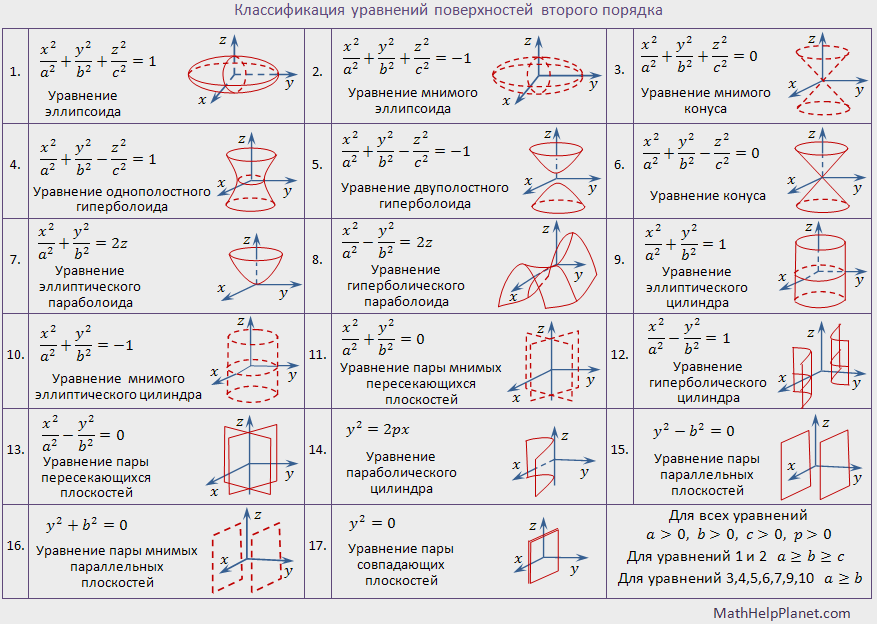
\includegraphics[width=\textwidth]{img/lines.png}
    \end{figure}

    Седьмое задание с экзамена 2019го года, вариант 2. 
    
    Найдите прямоугольную декартову систему координат в $\RR^3$ (выражение старых координат через новые), в которой уравнение поверхности
    \begin{equation*}
        2y^2 - 3z^2 + 4xz - 12y + 15 = 0
    \end{equation*}

    имеет канонический вид. Укажите этот вид, определите тип поверхности и нарисуйте её эскиз.

    \begin{solution}
        Выделим квадратную часть
        \begin{equation*}
            Q(x, y, z) = 2y^2 - 3z^2 + 4xz.
        \end{equation*}

        Приведем её к каноническому виду. Для этого воспользуемся алгоритмом приведения к главным осям. Найдем матрицу билинейной формы:
        \begin{equation*}
            B = \begin{pmatrix}
                0 & 0 & 2 \\
                0 & 2 & 0 \\
                2 & 0 & -3 \\
            \end{pmatrix}.
        \end{equation*}

        Найдем характеристический многочлен:
        \begin{equation*}
            \chi_B(t) = - \begin{vmatrix}
                -t & 0 & 2 \\
                0 & 2 - t & 0 \\
                2 & 0 & -3 - t \\
            \end{vmatrix}
            = t \cdot (2 - t) \cdot (-3 - t) + 4 \cdot (2 - t) = 0 \implies (t - 2) \cdot (t - 1) \cdot (t + 4) = 0.
        \end{equation*}

        Для каждого собственного значения находим его собственное подпространство (сразу нормируем векторы):
        \begin{itemize}
        \item[\pmb{$t = 1$}]
            \begin{equation*}
                \begin{pmatrix}
                    -1 & 0 & 2 \\
                    0 & 1 & 0 \\
                    2 & 0 & -4 \\
                \end{pmatrix}
                \to
                \begin{pmatrix}
                    1 & 0 & -2 \\
                    0 & 1 & 0 \\
                    0 & 0 & 0 \\
                \end{pmatrix}.
            \end{equation*}

            Отсюда $v_1 = \dfrac{1}{\sqrt{5}} \cdot (2, 0, 1)$.

        \item[\pmb{$t = 2$}]
            \begin{equation*}
                \begin{pmatrix}
                    -2 & 0 & 2 \\
                    0 & 0 & 0 \\
                    2 & 0 & -5 \\
                \end{pmatrix}
                \to
                \begin{pmatrix}
                    1 & 0 & 0 \\
                    0 & 0 & 1 \\
                    0 & 0 & 0 \\
                \end{pmatrix}.
            \end{equation*}

            Отсюда $v_2 = (0, 1, 0)$.

        \item[\pmb{$t = -4$}]
            \begin{equation*}
                \begin{pmatrix}
                    4 & 0 & 2 \\
                    0 & 6 & 0 \\
                    2 & 0 & 1 \\
                \end{pmatrix}
                \to
                \begin{pmatrix}
                    1 & 0 & 1/2 \\
                    0 & 1 & 0 \\
                    0 & 0 & 0 \\
                \end{pmatrix}.
            \end{equation*}

            Откуда $v_3 = \dfrac{1}{\sqrt{5}}(1, 0, -2)$.
        \end{itemize}

        Тогда в базисе $(v_1, v_2, v_3)$ квадратичная форма имеет вид
        \begin{equation*}
            Q(x', y', z') = x'^2 + 2y'^2 - 4z'^2.
        \end{equation*}

        Можно выразить старые координаты $(x, y, z)$ через новые координаты $(x', y', z')$:
        \begin{equation*}
            \begin{pmatrix}
                x \\ y \\ z \\
            \end{pmatrix}
            = \begin{pmatrix}
                v_1 & v_2 & v_3 \\
            \end{pmatrix}
            \cdot
            \begin{pmatrix}
                x' \\ y' \\ z' \\
            \end{pmatrix}
            = \begin{pmatrix}
                 2/\sqrt{5} & 0 & 1/\sqrt{5} \\
                 0 & 1 & 0 \\
                 1/\sqrt{5} & 0 & -2/\sqrt{5} \\
            \end{pmatrix}
            \cdot
            \begin{pmatrix}
                x' \\ y' \\ z' \\
            \end{pmatrix}.
        \end{equation*}

        Выражаем старые координаты явно:
        \begin{equation*}
            \colorbox{green!30}{$x = \dfrac{2}{\sqrt{5}}x' + \dfrac{1}{\sqrt{5}}z'$}; \quad \quad
            \colorbox{orange!30}{$y = y'$}; \quad \quad
            \colorbox{blue!30}{$z = \dfrac{1}{\sqrt{5}}x' - \dfrac{2}{\sqrt{5}}z'$}.
        \end{equation*}

        Подставляем в исходное выражение:
        \begin{align*}
            0
            &= 2y^2 - 3z^2 + 4xz - 12y + 15 \\
            &= x'^2 + 2y'^2 - 4z'^2 - 12y' + 15 \\
            &= x'^2 + 2(y'^2 - 6y' + 9) - 4z'^2 - 3 \\
            &= x'^2 + 2\left(y' - 3\right)^2 - 4z'^2 - 3 \\
        \end{align*}

        Заменяем $y' - 3$ одной переменной. Дальше каждую координату делим на константу, чтобы все коэффициенты в уравнении стали $\pm 1$. Получаем следующее выражение:
        \begin{equation*}
            \dfrac{(x'')^2}{3} + \dfrac{(y'')^2}{3/2} - \dfrac{(z'')^2}{3/4} = 1.
        \end{equation*}

        Смотрим на таблицу в начале секции. Это уравнение задает однополостной гиперболоид.
    \end{solution}

    \newpage
    \section{Нахождение жордановой формы линейного оператора и соответствующего жорданова базиса (К 41.1, 41.10, П 1530–1536).}

    Здесь будут полезны \href{https://docviewer.yandex.ru/view/286099993/?page=6&*=jIcVsIVsH1RJQlAqGKv0ADy944t7InVybCI6InlhLWRpc2stcHVibGljOi8vNi9YWE5ad2NSd3pjcnh0WVJ5NXBhWHIyOXJuNkhDV3dMUWdDY2RHYW5Qb2t0RDEvM0hvT1ZTRDFOV2cvVHVPbnEvSjZicG1SeU9Kb25UM1ZvWG5EYWc9PTovYWxnb3JpdGhtcy5wZGYiLCJ0aXRsZSI6ImFsZ29yaXRobXMucGRmIiwibm9pZnJhbWUiOmZhbHNlLCJ1aWQiOiIyODYwOTk5OTMiLCJ0cyI6MTU5MTk2ODE4NjIyMiwieXUiOiI1NDI5NTAxMzQxNTY1NTI2MzYyIn0%3D}{алгоритмы} Димы начиная с 19го.


    Восьмое задание с экзамена 2019го года, вариант 1. Спонсор решения --- Сабина Даянова.

    Линейный оператор $\phi: \RR^4 \to \RR^4$ имеет в стандартном базисе матрицу
    \begin{equation*}
        A = \begin{pmatrix}
            2 & 1 & 0 & -2 \\
            0 & 1 & 0 & 2 \\
            3 & 4 & 2 & -5 \\
            0 & -1 & 0 & 4 \\
        \end{pmatrix}.
    \end{equation*}

    Найдите базис в пространстве $\RR^4$, в котором матрица оператора $\phi$ имеет жорданову форму, и укажите эту жорданову форму.

    \begin{solution}
        Сначала надо найти собственные значения этого оператора. Для этого найдем корни характеристического многочлена. Определитель будем раскладывать по первому столбцу, так как тогда будет только одно ненулевое слагаемое:
        \begin{equation*}
            \chi_{\phi}(t) = \det(A - t \cdot E) = (t - 2) \cdot \begin{vmatrix}
                1 - t & 0 & 2 \\
                4 & 2 - t & -5 \\
                -1 & 0 & 4 - t \\
            \end{vmatrix} = (t - 2)^3 (t - 3) = 0.
        \end{equation*}

        Различные собственные значения можно рассматривать по отдельности. Оператор принимает одну из следующих конфигураций:
        \begin{equation*}
            \begin{pmatrix}
                3 & & & \\
                & 2 & & \\
                & & 2 & \\
                & & & 2 \\
            \end{pmatrix}; \quad \quad
            \begin{pmatrix}
                3 & & & \\
                & 2 & 1 & \\
                & & 2 & \\
                & & & 2\\
            \end{pmatrix}; \quad \quad
            \begin{pmatrix}
                3 & & & \\
                & 2 & 1 & \\
                & & 2 & 1\\
                & & & 2 \\
            \end{pmatrix}.
        \end{equation*}

        \begin{options}
        \item 
            Для собственного значения $3$ получаем, что есть только одна клетка размера $1$.

        \item 
            Для собственного значения $2$ суммарный размер клеток должен равняться $3$. Тогда возможны следующие конфигурации:
            \begin{itemize}
            \item 
                $3$ клетки размера $1$;
            \item
                $1$ клетка размера $1$, $1$ клетка размера $2$;
            \item 
                $1$ клетка размера $3$.
            \end{itemize}

            Знаем, что число клеток размера $k$ вычисляется по следующей формуле:
            \begin{equation*}
                \rk(A - \lambda \cdot E)^{k + 1} + \rk(A - \lambda \cdot E)^{k - 1} - 2 \cdot \rk(A - \lambda \cdot E)^k.
            \end{equation*}

            Или, если $r_s = \rk(A - \lambda \cdot E)^s$, то $r_{s + 1} + r_{s - 1} - 2 \cdot r_s$.

            Количество клеток размера $1$ однозначно определяет конфигурацию в нашем случае. Найдем $r_i$:
            \begin{align*}
                r_0 &= \rk E = 4; \\
                r_1 &= \rk(A - 2 \cdot E) = \rk \begin{pmatrix}
                    0 & 1 & 0 & -2 \\
                    0 & -1 & 0 & 2 \\
                    3 & 4 & 0 & -5 \\
                    0 & -1 & 0 & 2 \\
                \end{pmatrix}
                =
                \rk \begin{pmatrix}
                    3 & 4 & 0 & -5 \\
                    0 & 1 & 0 & -2 \\
                    0 & 0 & 0 & 0 \\
                    0 & 0 & 0 & 0 \\
                \end{pmatrix}
                =
                \rk \begin{pmatrix}
                    1 & 0 & 0 & 1 \\
                    0 & 1 & 0 & -2 \\
                    0 & 0 & 0 & 0 \\
                    0 & 0 & 0 & 0 \\
                \end{pmatrix}
                = 2; \\
                r_2 &= \rk (A - 2 \cdot E)^2
                =
                \rk \begin{pmatrix}
                    0 & 1 & 0 & -2 \\
                    0 & -1 & 0 & 2 \\
                    0 & 4 & 0 & -8 \\
                    0 & -1 & 0 & 2 \\
                \end{pmatrix}
                = \rk \begin{pmatrix}
                    0 & 1 & 0 & -2 \\
                    0 & 0 & 0 & 0 \\
                    0 & 0 & 0 & 0 \\
                    0 & 0 & 0 & 0 \\
                \end{pmatrix}
                = 1.
            \end{align*}

            Тогда для собственного значения $2$ имеем $1 + 4 - 2 \cdot 2 = 1$ клетку размера $1$. Автоматически получаем, что есть еще одна клетка размера $2$. 
        \end{options}

        Получили следующую Жорданову матрицу:
        \begin{equation*}
            \begin{pmatrix}
                3 & & & \\
                & 2 & 1 & \\
                & & 2 & \\
                & & & 2\\
            \end{pmatrix}.
        \end{equation*}

        Так как мы привели матрицы к ступенчатому виду, легко найти ФСР.
        \begin{options}
        \item 
            ФСР у $(A - 2 \cdot E) \cdot x = 0$:
            \begin{equation*}
                v_1 = (0, 0, 1, 0); \quad
                v_2 = (-1, 2, 0, 1).
            \end{equation*}

            Заметим, что эти векторы являются собственными для собственного значения $2$.

        \item 
            ФСР у $(A - 2 \cdot E)^2 \cdot x = 0$:
            \begin{equation*}
                u_1 = (1, 0, 0, 0); \quad
                u_2 = (0, 0, 1, 0); \quad
                u_3 = (0, 2, 0, 1).
            \end{equation*}
        \end{options}

        Теперь необходимо найти базис. Обозначим его за $(w_1, w_2, w_3, w_4)$.

        \begin{options}
        \item 
            $w_1$ --- это собственный вектор для собственного значения $3$. Найдем его из ФСР $(A - 3 \cdot E) \cdot x = 0$:
            \begin{equation*}
                \begin{pmatrix}
                    -1 & 1 & 0 & -2 \\
                    0 & -2 & 0 & 2 \\
                    3 & 4 & -1 & -5 \\
                    0 & -1 & 0 & 1 \\
                \end{pmatrix}
                \to
                \begin{pmatrix}
                    1 & -1 & 0 & 2 \\
                    0 & -1 & 0 & 1 \\
                    0 & -2 & 0 & 2 \\
                    0 & 7 & -1 & -11 \\
                \end{pmatrix}
                \to
                \begin{pmatrix}
                    1 & -1 & 0 & 2 \\
                    0 & 1 & 0 & -1 \\
                    0 & 0 & 1 & 4 \\
                    0 & 0 & 0 & 0 \\
                \end{pmatrix}
                \to
                \begin{pmatrix}
                    1 & 0 & 0 & 1 \\
                    0 & 1 & 0 & -1 \\
                    0 & 0 & 1 & 4 \\
                    0 & 0 & 0 & 0 \\
                \end{pmatrix}.
            \end{equation*}

            Отсюда \colorbox{blue!30}{$w_4 = (-1, 1, -4, 1)$}.

        \item 
            $w_2$ и $w_4$ --- это собственные векторы для собственного значения $2$. Заметим, что
            \begin{equation*}
                w_3 \notin \ker (A - 2 \cdot E); \quad
                w_3 \in \ker (A - 2 \cdot E)^2.
            \end{equation*}

            Например, \colorbox{green!30}{$w_3 = (1, 0, 0, 0)$}.

            Но мы знаем, что $A \cdot w_3 = 2w_3 + w_2$ (потому что мы в стандартном базисе). Тогда \colorbox{red!30}{$w_2 = (A - 2 \cdot E) \cdot w_3 = (0, 0, 3, 0)$}. Тогда \colorbox{orange!30}{$w_4 = (-1, 2, 0, 1)$}.
        \end{options}

        Не забываем проверить в конце полученный базис на линейную назависимость.
    \end{solution}
\end{document}